% =============================================================================
% Section 11 — Closing the Gaps
% =============================================================================
\section{Closing the Gaps: Topology, Homology and Interaction}\label{sec:gaps}

\begin{objectives}
\begin{itemize}[leftmargin=*,itemsep=1pt,topsep=1pt]
  \item Run the shuffle null that decides whether a topological feature is biology or embedding.
  \item Read a negative result as a result, and distinguish it from an absence of work.
  \item Verify an orthologous residue correspondence instead of assuming it, and identify which statistic carries the evidence.
  \item Price an escape route: turn ``perhaps the stages interact'' into an inequality a measurement can check.
\end{itemize}
\end{objectives}

\subsection{Why this section exists}

Every section so far ends with a ledger, and every ledger has an \textbf{Open}
line. A ledger that never discharges anything is not a discipline; it is a
disclaimer with good manners. This section discharges four of those lines.

Three of them are closed by work that could have come out the other way, which
is the only kind worth reporting:

\begin{enumerate}[leftmargin=*,itemsep=2pt]
  \item \textbf{Section~\ref{sec:tda}} computed persistent homology on the
        \texttt{POLE} coding sequence, then declined to draw any biological
        conclusion because no null was run. The null is now run. It comes out
        negative, and that is the finding.
  \item \textbf{Section~\ref{sec:variants}} assumed that yeast \texttt{pol2-P301R}
        models human \texttt{P286R}. It is now verified by alignment --- and the
        verification changes which statistic one should quote.
  \item \textbf{Section~\ref{sec:nogo}} left one escape route from the no-go
        theorem: stages that interact are not covered by
        Assumption~\ref{model:class}. The route is now priced.
  \item \textbf{Section~\ref{sec:mmr}}'s transport problem
        (Remark~\ref{rem:transport}) is turned from a caveat into a pair of
        machine-checked theorems, one of which is a counterexample.
\end{enumerate}

\subsection{Is the topology biology? A shuffle null}\label{sub:tdanull}

Section~\ref{sec:tda} argued that the chaos game sends any sequence into a
self-similar attractor whose holes exist regardless of what the sequence says,
and that the Betti numbers of a single sequence therefore carry almost no
biological information. That was an assertion. Here it is a measurement.

\begin{model}[The test]\label{model:tdanull}
The statistic is the \emph{total persistence} of $H_1$: the sum of the lengths of
all finite $H_1$ bars in the Vietoris--Rips filtration of the chaos-game cloud.
It is compared against three nested nulls, each destroying one more level of
sequence structure while preserving the level below:
\begin{itemize}[leftmargin=*,itemsep=1pt,topsep=1pt]
  \item \textbf{mono} --- a uniform permutation. Preserves base composition,
        destroys every $k$-mer statistic for $k \ge 2$.
  \item \textbf{dinuc} --- an Altschul--Erickson Eulerian-path shuffle. Preserves
        every dinucleotide count \emph{exactly}, destroys $k \ge 3$.
  \item \textbf{codon} --- a permutation of whole codons. Preserves codon usage
        and the reading frame, destroys codon order.
\end{itemize}
\end{model}

Reading the three together localises any signal. A sequence that beats
\textbf{mono} but not \textbf{dinuc} has dinucleotide structure and nothing
above it; one that beats \textbf{dinuc} but not \textbf{codon} has structure that
codon usage explains.

\begin{numerics}[11.1]
\file{scripts/textbook/tda_sequence_null.py}. $200$ shuffles per null, $500$
points, maximum edge length $0.8$, seed \texttt{20261022}. Empirical two-sided
$p$-values with the observation included, so the attainable floor is
$2/201 = 0.010$ and is reported rather than implied.

Three coding sequences were tested, which also supplies the cross-sequence
comparison Section~\ref{sec:tda} left undone. Subsampling strides are $13$, $5$
and $8$, all coprime with the codon period for the reason
\S\ref{sub:strideartefact} explains at length.

\medskip
\begin{tabularx}{\linewidth}{@{}l l r r r X@{}}
\toprule
\textbf{Gene} & \textbf{Null} & \textbf{observed} & \textbf{null mean} & \textbf{$z$} & \textbf{$p$ (two-sided)} \\
\midrule
\texttt{POLE}  & mono  & $5.293$ & $6.218$ & $-1.64$ & $0.099$ \\
               & dinuc & $5.293$ & $5.549$ & $-0.50$ & $0.627$ \\
               & codon & $5.293$ & $5.780$ & $-0.92$ & $0.428$ \\
\midrule
\texttt{POLD1} & mono  & $5.007$ & $5.444$ & $-0.83$ & $0.408$ \\
               & dinuc & $5.007$ & $4.897$ & $+0.26$ & $0.945$ \\
               & codon & $5.007$ & $4.889$ & $+0.26$ & $0.856$ \\
\midrule
\texttt{MSH6}  & mono  & $5.173$ & $6.149$ & $-1.79$ & $0.060$ \\
               & dinuc & $5.173$ & $5.726$ & $-1.01$ & $0.358$ \\
               & codon & $5.173$ & $6.019$ & $-1.53$ & $0.159$ \\
\bottomrule
\end{tabularx}
\end{numerics}

\begin{figure}[htbp]
  \centering
  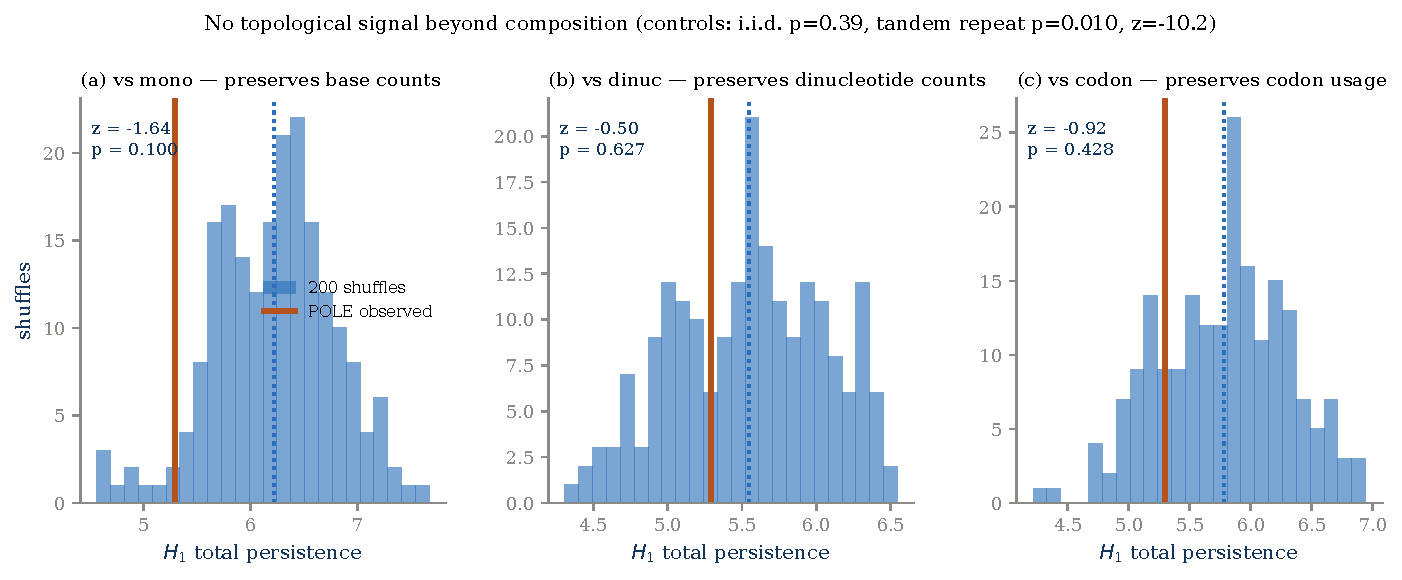
\includegraphics[width=\textwidth]{fig11_tda_null.pdf}
  \caption{The shuffle null for the \texttt{POLE} coding sequence. Each
  histogram is $200$ actual shuffle draws --- not a Gaussian fitted to two
  moments --- with the observed value in orange. The observed total persistence
  sits inside every null. Against \textbf{mono} it is $1.6$ standard deviations
  \emph{below} the null mean, and that modest displacement is fully absorbed once
  dinucleotide composition is preserved. Generated by
  \file{scripts/textbook/make_figures.py}, section~11, from
  \file{data/tda_sequence_null.json}.}
  \label{fig:tdanull}
\end{figure}

\subsubsection*{The result, stated plainly}

None of the three coding sequences shows a signal: every $p$ exceeds $0.05$, and
the largest displacement anywhere in the table is $1.8$ standard deviations. In
particular the \texttt{POLE} coding sequence has \textbf{no detectable topological signal
beyond its base composition}. Section~\ref{sec:tda}'s caution was correct, and
it is now earned rather than asserted.

Two details are worth more than the headline.

First, the displacement is \emph{negative}: the real sequence has slightly
\emph{less} $H_1$ persistence than its shuffles. Had we gone looking for
``structure'' we would have been looking in the wrong direction. A one-sided test
chosen after seeing the data would have reported $p \approx 0.95$ and we might
have called that a clean null; the two-sided test reports $0.099$, which is the
honest number and is still not significant.

Second, the mono-to-dinuc comparison localises what little there is. The $z$ of
$-1.64$ against \textbf{mono} falls to $-0.50$ against \textbf{dinuc}, so
whatever weak tendency exists is a \emph{dinucleotide composition} effect, not
higher-order sequence structure. That is a more informative negative than a bare
``not significant'', and it is only available because the nulls were nested.

\subsection{The artefact this section made, and how it was caught}\label{sub:strideartefact}

The first run of the experiment above reported a different result, and the way it
was wrong is more instructive than the corrected numbers.

\texttt{POLD1} appeared to carry a strongly significant signal: against the
mononucleotide null, $z = -3.59$ at the attainable $p$ floor of $0.010$, and
against the dinucleotide null $z = -2.90$, $p = 0.020$. Taken at face value this
was a genuine cross-sequence finding --- topological structure in one replicative
polymerase gene and not another --- and it is the sort of result one is tempted
to write up.

It was an artefact of our own sampling, and this book had already warned about
it. Worked Example~8.1 says, in those words, that a subsampling stride sharing a
factor with the reading frame over-samples one codon position, and that a stride
of $6$ or $9$ ``would have introduced a frame bias invisible in the final
diagram''. \texttt{POLD1}'s coding sequence is $3324$~nt, the subsample takes
$500$ points, and $3324 / 500$ rounds down to a stride of exactly $6$.

\begin{remark}[Why a frame-biased stride manufactures a signal]
The mechanism is worth following, because it explains both the false positive and
the clue that exposed it.

A stride of $6$ on a coding sequence visits only codon position~$1$, over and
over. Codon position~$1$ has its own base composition, markedly different from
the gene's overall composition. So the \emph{observed} cloud is built from a
compositionally skewed subsequence --- while the \textbf{mono} and \textbf{dinuc}
shuffles have no reading frame left to be biased by, and their clouds are built
from compositionally representative samples. Observed and null are then not
comparable, and the difference shows up as a displacement in total persistence.

Now the clue. The \textbf{codon} null permutes whole codons, so it
\emph{preserves} the reading frame --- and therefore suffers the identical
sampling bias. Against that null the bias cancels on both sides, and sure enough
\texttt{POLD1} gave $z = -0.44$, $p = 0.607$: no signal at all.

A finding that survives two nulls and vanishes against the third, where the
third is the only one preserving the frame, is not a finding about biology. It is
a signature, and reading it correctly requires having designed the nulls to be
nested in the first place.
\end{remark}

The fix is one line --- the stride is now chosen coprime with $3$, giving $13$
for \texttt{POLE}, $5$ for \texttt{POLD1} and $8$ for \texttt{MSH6} --- and it is
asserted in the script and in \file{tests/test_tda_null_and_orthologue.py}, so a
future change of point count cannot silently reintroduce it. Re-running is a
controlled comparison, because only \texttt{POLD1}'s stride changes: \texttt{POLE}
and \texttt{MSH6} were already coprime, so their numbers and the controls' must
come out identical, and they do. \texttt{POLD1}'s apparent signal does not
survive:

\medskip
\noindent
\texttt{POLD1}, $z$ of the $H_1$ total persistence against each null, before and
after the stride was made frame-safe:

\medskip
\begin{tabular}{@{}l r r r l@{}}
\toprule
\textbf{null} & \textbf{stride 6} & \textbf{stride 5} & \textbf{$p$} & \textbf{reading} \\
\midrule
mono  & $-3.59$ & $-0.83$ & $0.408$ & signal gone \\
dinuc & $-2.90$ & $+0.26$ & $0.945$ & signal gone \\
codon & $-0.44$ & $+0.26$ & $0.856$ & no signal either way \\
\bottomrule
\end{tabular}

\medskip
\noindent
The observed statistic itself moves, from $3.577$ to $5.007$, which is the direct
evidence that the biased stride was sampling a compositionally \emph{different}
subsequence and not merely a smaller one. Note also that the \textbf{codon} row's
$z$ changes, from $-0.44$ to $+0.26$: the prediction was never that this number
would stay fixed, but that it would show no signal in \emph{either} run, because
there the bias afflicts observed and null alike. It is the only row of which that
was true beforehand, and that is exactly why the artefact was visible.

\medskip
Three things are worth taking from this.

\emph{The warning was already in the book and did not prevent the error.} Knowing
about an artefact in the abstract is not the same as checking for it in your own
pipeline. The check is now code, not prose, which is the only form that
generalises.

\emph{The nested design did the work.} Had we run a single shuffle null --- the
usual practice --- the \texttt{POLD1} result would have been significant,
plausible and wrong, with nothing in the output to suggest otherwise. The third
null was not redundancy; it was the diagnostic.

\emph{The temptation ran the right way for once.} A spurious positive is easier
to publish than the negative result it displaced, and the only reason it was
examined at all is that it was surprising. That is a thin safeguard, and it is
why the stride is now asserted rather than inspected.

\begin{ledger}[Controls, because a null result is only as good as its power]
A null test that cannot come out positive is worthless, so both directions were
checked and both are asserted in code --- the script exits non-zero and writes
nothing if either fails.

\textbf{Negative control:} an i.i.d.\ sequence drawn from the real base
frequencies, which has no structure above composition by construction. Against
\textbf{mono} it gives $p = 0.388$, $z = +0.90$. Not flagged, as required: the
test does not manufacture signal.

\textbf{Positive control:} a tandem repeat of a single motif, composition-matched
to the real sequence so that only its \emph{order} differs. Against \textbf{mono}
it gives $p = 0.010$ --- the attainable floor --- at $z = -10.17$. Flagged
overwhelmingly, as required: the test has power to detect order.

So the negative result above is informative. A test that flagged a tandem repeat
at $z = -10$ and the real sequence at $z = -1.6$ is telling us something about
the sequence, not about its own insensitivity.
\end{ledger}

\subsection{Is yeast \texttt{P301} really human \texttt{P286}?}\label{sub:ortho}

The refutation of Section~\ref{sec:refutation} runs entirely through a yeast
allele. If \texttt{pol2-P301R} is not the structural analogue of human
\texttt{P286R}, the chain breaks at its first link --- and the book assumed the
correspondence without checking it.

\begin{numerics}[11.2]
\file{scripts/textbook/verify_yeast_human_correspondence.py}. Full-length global
alignment (Gotoh, affine gaps) of human \texttt{POLE} (UniProt \texttt{Q07864},
$2286$~aa) against \emph{S.~cerevisiae} \texttt{POL2} (\texttt{P21951},
$2222$~aa), both retrieved live with URLs and a UTC timestamp.

We have no verified substitution matrix on this host, and transcribing one from
memory is the kind of unchecked assertion this book argues against. So the
alignment is run under four explicit scoring schemes and gap costs, and the
result is reported only as \emph{invariant across them}. Human residue $286$
aligns to yeast residue $301$ in all four, at $43.1$--$44.8\%$ global identity.
\end{numerics}

The aligned neighbourhood is the real evidence, and it is worth printing:

\begin{center}
\begin{tabular}{@{}l l@{}}
human \texttt{POLE} $279$--$293$  & \texttt{T K L P L K F \textbf{P} D A E T D Q I} \\
yeast \texttt{POL2}\ $294$--$308$ & \texttt{T K P P L K F \textbf{P} D S A V D Q I} \\
\end{tabular}
\end{center}

\noindent
Eleven of fifteen positions are identical, and the substituted residue sits
inside an exactly conserved \texttt{F-P-D} tripeptide: human
$\texttt{F}285\,\texttt{P}286\,\texttt{D}287$ against yeast
$\texttt{F}300\,\texttt{P}301\,\texttt{D}302$. This is the ExoI motif, whose
aspartate is one of the two catalytic carboxylates that \texttt{pol2-4} replaces
with alanine.

\begin{figure}[htbp]
  \centering
  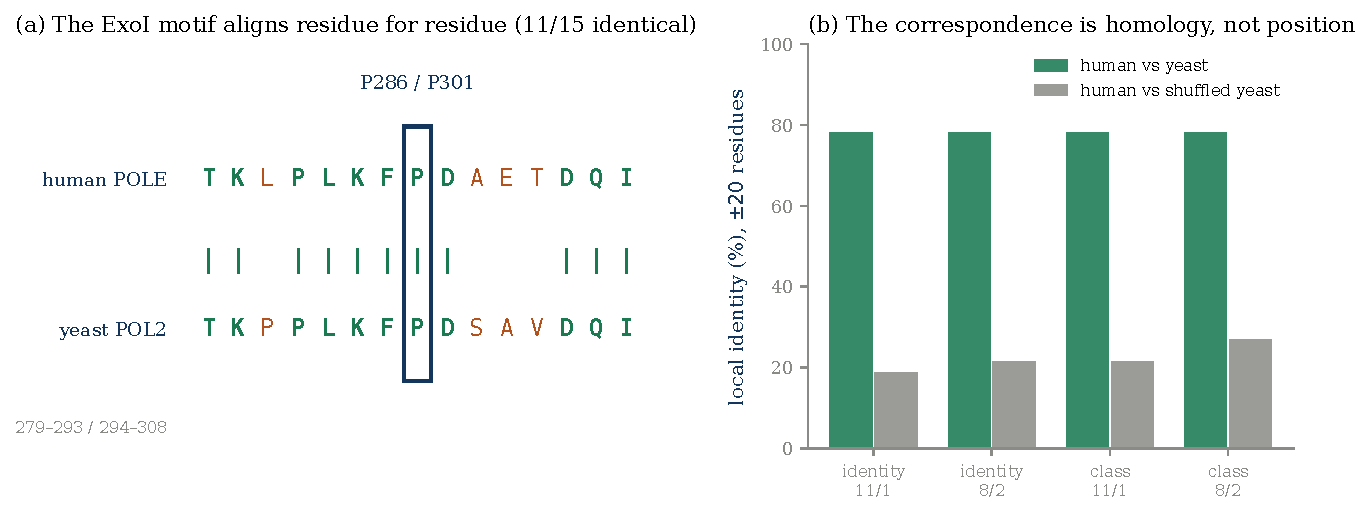
\includegraphics[width=\textwidth]{fig12_orthologue_alignment.pdf}
  \caption{(a) The aligned ExoI neighbourhood, residue by residue; green where
  identical. The boxed column is the substituted proline. (b) Local identity in
  a $\pm20$-residue window about the site, for the real pair against a
  composition-matched shuffle of the yeast sequence, under each scoring scheme.
  The real pair holds at $78.0\%$ throughout; the shuffle reaches at most
  $26.8\%$.}
  \label{fig:ortho}
\end{figure}

\begin{remark}[Which statistic actually carries the evidence]\label{rem:diagonal}
Here the verification taught us something we would have got wrong.

The obvious thing to report is ``human $286$ aligns to yeast $301$''. But that
claim is weaker than it looks, and the negative control shows why: aligning
human \texttt{POLE} against a \emph{shuffled} yeast sequence maps residue $286$
to residue $302$ --- one position away from the right answer. A global alignment
of two sequences of similar length follows the diagonal whatever the sequences
say, so positional agreement is largely a fact about the two lengths.

The statistic with no such prior is \emph{local conservation}. Around the site
the real pair holds $78.0\%$ identity against the shuffle's $26.8\%$, a factor of
$2.9$, under every scheme. That is the number the script gates on, and it is the
number a reader should be given.

The general lesson is the one from Section~\ref{sec:proof-and-cell} in a new
costume: ask what the control could have produced. A control that returns $302$
when the answer is $301$ has not validated anything, and quoting the position as
the result would have hidden that.
\end{remark}

So the correspondence holds. Note exactly what has been established: that the
two residues occupy the same position in a conserved motif. That is a claim about
sequence, and it is what the book needed. It is \emph{not} a claim that the two
enzymes respond identically to the substitution, which no alignment can settle.

\subsection{What if the stages interact?}\label{sub:interact}

Section~\ref{sec:nogo}'s ledger named one escape route from the no-go theorem,
and named it honestly: Assumption~\ref{model:class} requires stages to compose
multiplicatively and independently, and a model in which they \emph{interact} is
not covered. A reader could reasonably have replied: ``then the refutation only
kills the independent case, and you have not told me how much interaction it
would take to survive.''

That is a fair objection, and it has a number for an answer.

\begin{model}[Interacting stages]\label{model:interact}
Carry an explicit interaction factor $\Lambda \ge 0$:
\begin{equation}\label{eq:interact}
  \errate_\Lambda(\stages) \;=\; \inserr \Big(\prod_{i \in \stages} \escape_i\Big)\,\Lambda .
\end{equation}
$\Lambda = 1$ is exactly the independent class of Section~\ref{sec:nogo};
$\Lambda > 1$ says that losing stages is worse than multiplicativity predicts,
which is what ``the stages interact'' means quantitatively.
\end{model}

\begin{theorem}[The interacting ceiling, PSR$_2$I]\label{thm:psr2i}
Under the hypotheses of Assumption~\ref{model:class} together with
\eqref{eq:interact} and $\Lambda \ge 0$,
$\;\errate_\Lambda(\stages) \le \inserr\Lambda$ for every $\stages$.
\end{theorem}

\begin{proof}
The product lies in $[0,1]$, so $\inserr\prod \escape_i \le \inserr$; multiplying
by $\Lambda \ge 0$ preserves the inequality.
\end{proof}

\begin{theorem}[The price of the rescue, PSR$_3$I]\label{thm:psr3i}
If a variant keeping stages $\kept$ is measured at $\rho$ times the
exonuclease-null error, with $\inserr > 0$, then $\rho \le \Lambda$.
\end{theorem}

\begin{proof}
By Theorem~\ref{thm:psr2i} the observed rate $\rho\inserr$ is at most
$\inserr\Lambda$. Divide by $\inserr > 0$.
\end{proof}

\begin{figure}[htbp]
  \centering
  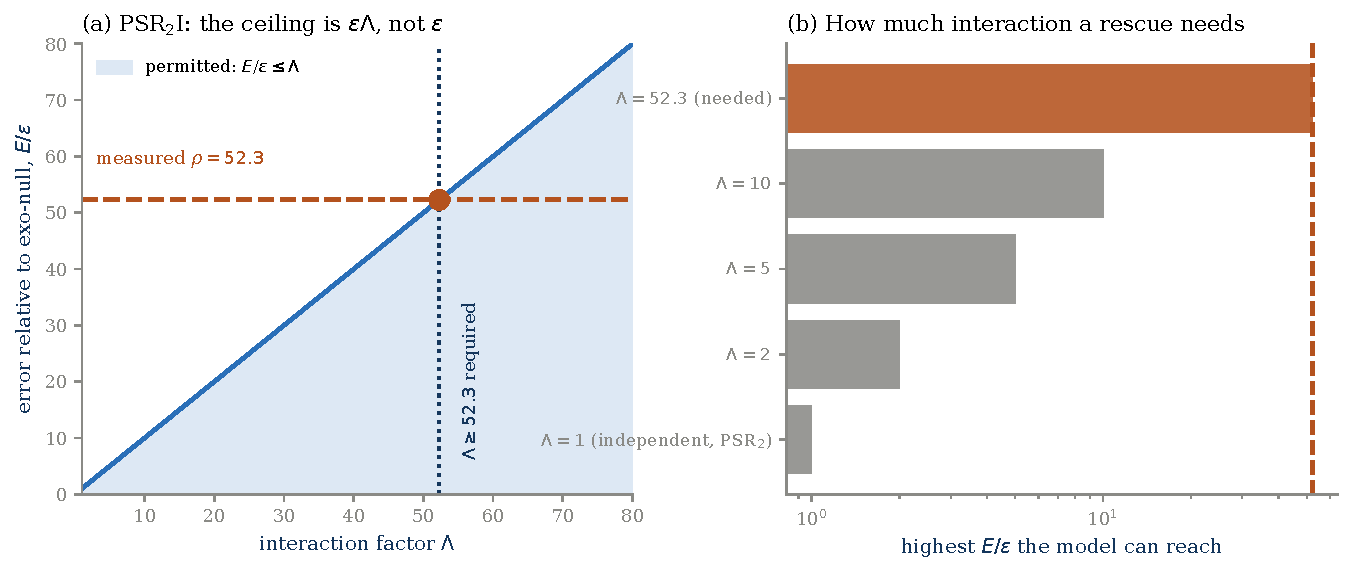
\includegraphics[width=\textwidth]{fig13_interaction_price.pdf}
  \caption{(a) The interacting ceiling. The permitted region is
  $\errate/\inserr \le \Lambda$; the measured $\rho = 52.3$ forces
  $\Lambda \ge 52.3$. (b) What each level of interaction can reach. The
  independent class of Section~\ref{sec:nogo} is the $\Lambda = 1$ bar, where the
  original ceiling returns.}
  \label{fig:interaction}
\end{figure}

\noindent
Put the measurement in. With $\rho = 2300/44 = 52.3$:

\begin{center}
\emph{A stage-removal account of \texttt{pol2-P301R} requires stages whose
interaction makes their loss at least $52$ times more damaging than independence
allows.}
\end{center}

This does not refute the interacting class, and it is important not to pretend
otherwise. What it does is convert a qualitative escape hatch into a
quantitative claim that an enzymologist can assess: is there any mechanism by
which three proofreading stages cooperate so strongly that removing them is
fifty-two-fold worse than their product? The question is now answerable, which it
was not before. Converting an unfalsifiable objection into a falsifiable one is
the whole service this book claims for formal methods, and here it is being
performed on an objection to the book's own argument.

\subsection{Formalisation}

\file{formal/ANSE/InteractingStagesAndTransport.lean}, $11$ of $11$ declarations
clean on the axiom gate.

\begin{lstlisting}
noncomputable def errorRateI {ι : Type*} (ε : ℝ) (q : ι → ℝ) (S : Finset ι)
    (Λ : ℝ) : ℝ := ε * (∏ i ∈ S, q i) * Λ

theorem PSR_3I_excess_forces_interaction {ι : Type*}
    (ε ρ Λ : ℝ) (hε : 0 < ε) (q : ι → ℝ)
    (h0 : ∀ i, 0 ≤ q i) (h1 : ∀ i, q i ≤ 1)
    (T : Finset ι) (hΛ : 0 ≤ Λ)
    (hobs : errorRateI ε q T Λ = ρ * ε) : ρ ≤ Λ
\end{lstlisting}

\noindent
The module also carries \lean{psr2I_recovers_psr2}, which shows the original
ceiling returns at $\Lambda = 1$ --- the control confirming that $\Lambda$ is
load-bearing and not decoration --- and
\lean{interaction_hypotheses_satisfiable}, a witness that the hypotheses of
Theorem~\ref{thm:psr3i} are jointly satisfiable with a nontrivial product and
$\rho > 1$. Without the witness the theorem could hold merely because nothing
meets its assumptions.

\subsubsection*{The transport problem, as a theorem}

Remark~\ref{rem:transport} argued that Section~\ref{sec:mmr}'s conclusion rests
on carrying an in vitro inequality into a cell. That was prose. The same module
makes it arithmetic. Writing production as
$\mathrm{prod}(e,s) = e\cdot s$, with $e$ the error rate per nucleotide and $s$
the nucleotides synthesised per replicated genome:

\begin{lstlisting}
theorem per_nucleotide_does_not_transport :
    ∃ eMut eNull sMut sNull : ℝ,
      0 ≤ eMut ∧ 0 ≤ eNull ∧ 0 ≤ sMut ∧ 0 ≤ sNull ∧
      eMut ≤ eNull ∧
      production eNull sNull < production eMut sMut

theorem transport_needs_synthesis_bound (eMut eNull sMut sNull : ℝ)
    (he0 : 0 ≤ eMut) (hs0 : 0 ≤ sMut)
    (he : eMut ≤ eNull) (hs : sMut ≤ sNull) :
    production eMut sMut ≤ production eNull sNull
\end{lstlisting}

The first is a counterexample, and the witness is the measured enzyme in
miniature: $e = 59$ against $155$, $s = 40$ against $4$. More accurate per
nucleotide, four times the delivered load. The second names the missing
hypothesis exactly --- $s_{\mathrm{mut}} \le s_{\mathrm{null}}$ --- and it is a
statement about how much of the genome each enzyme copies, which no experiment
in this book measures.

A caveat is now a theorem, which means it can no longer be forgotten.

\subsection{What the combination buys}\label{sub:combination}

This book has used machine-checked proof, exact and numerical computation, live
database retrieval, and computational topology on the same problem. It is worth
being precise about what each contributed, because the honest accounting is
uneven and the uneven parts are the instructive ones.

\begin{itemize}[leftmargin=*,itemsep=3pt]
  \item \textbf{Proof contributed the refutation.} PSR$_2$ has no free
        parameters, so one ratio killed a mechanism class. That is the single
        most consequential step in the book, and it was available only because
        the hypothesis had been stated precisely enough to be refuted.
  \item \textbf{Proof also contributed the limits of the refutation.}
        Theorem~\ref{thm:psr3i} prices the escape route;
        \lean{per_nucleotide_does_not_transport} exhibits the gap in the
        replacement mechanism. Formalisation was at least as useful pointed at
        our own conclusions as at the one we overturned.
  \item \textbf{Numerics contributed a correction.} The Luria--Delbrück
        simulation of Section~\ref{sec:accumulation} did not confirm the closed
        form; it exposed that the variance is not estimable at any feasible
        number of cultures (\S\ref{sub:trap}). The computation was useful
        precisely by disagreeing.
  \item \textbf{Retrieval contributed two corrections.} The live scripts caught
        a wrong assumption about ClinVar's categories partitioning, and a wrong
        source for domain boundaries. Both were our errors, found because the
        data were fetched and checked rather than quoted.
  \item \textbf{Topology contributed a negative result.} \S\ref{sub:tdanull} is
        the honest answer to the question Section~\ref{sec:tda} raised, and the
        answer is no. This is the most conspicuous case of a method producing a
        beautiful picture and no biological knowledge, and it is in the book for
        that reason.
\end{itemize}

\begin{remark}[The absent layer line, again]\label{rem:franklin-again}
It is worth noticing what kind of evidence this section's central result is,
because the book is dedicated to someone whose decisive evidence was of the same
kind.

Photo~51's contribution was in part an \emph{absence}: the fourth layer line is
missing, and \S\ref{sub:photo51} shows that a two-strand helix offset by
$\delta = 3/8$ requires it to be missing. An absence is only evidence if the
method could have shown the thing. Franklin's plate could --- the neighbouring
layer lines are plainly there, which is precisely why the gap at $n = 4$ means
something. Had the exposure been too short to show any layer lines, their absence
would have meant nothing at all.

\S\ref{sub:tdanull} is an absence of exactly this structure. The claim is that
\texttt{POLE} shows no topological signal beyond composition, and that claim is
worth something only because the same test flagged a composition-matched tandem
repeat at $z = -10.2$. The positive control plays the role the visible layer
lines play on the plate: it establishes that the method can see.

This is, we think, the most useful single habit in the book. A negative result
and an unperformed experiment produce the same number of significant findings,
and are told apart only by the control. State it, or the absence is just silence.
\end{remark}

\begin{remark}[On the temptation that topology presents]
It would have been easy to publish Figure~\ref{fig:tda} with a sentence about
``the intrinsic topological signature of the \texttt{POLE} locus'' and no null.
The picture is striking, the method is fashionable, and almost no reader checks.
Running the null cost an afternoon and produced a result that is harder to
publish and more worth having.

We single this out because the incentive gradient runs the wrong way, and a
student should know that in advance. The methods in this book that most readily
produce impressive output --- high-dimensional embeddings, persistence diagrams,
and anything with a $3$D rendering --- are exactly the ones whose nulls are most
often omitted.
\end{remark}

\subsection{The human stakes, stated carefully}

The user of a textbook is entitled to ask what any of this is for, and the
answer should not be inflated.

Nothing in this book has treated a patient. The refutation of
Section~\ref{sec:refutation} does not change the management of a
\texttt{POLE}-mutant tumour, and Section~\ref{sec:clinic} explains why the
clinical decision rule was never load-bearing on the mechanism. The topology is a
negative result. The alignment confirms something the field already assumed.

What has been produced is narrower and real: one retracted mechanism, a sharper
question about mismatch repair, a priced escape route, a named missing
measurement, and a worked demonstration that each of these can be found by
reading one's own claims adversarially.

The argument for the value of that is an argument about aggregate harm. Wrong
mechanisms in the biomedical literature are not harmless. They direct grant
money, select which experiments get done, and shape which variants a clinician
treats as explained. They persist because mechanisms are usually stated loosely
enough to accommodate contrary data --- and the remedy is not better intentions
but statements sharp enough to fail. Every retraction in this book was possible
only because something had been written down precisely.

The care for the people downstream, then, looks like this in practice: state the
mechanism as a model class, prove what the class entails without fitting,
compare against a directly measured reference, run the control that could
embarrass you, and publish the refutation when it comes --- including when it is
your own. It requires no new technology. It requires being willing to be wrong in
public, on the record, with the date attached.

That is the whole method. A student who takes nothing else from this book should
take the habit of asking, of every claim including their own: \emph{what would
have had to happen for this to come out differently?} If the answer is nothing,
there is no evidence there, however good the figure looks.

\begin{worked}[11.1: reading a negative result correctly]
\textbf{Problem.} A colleague summarises \S\ref{sub:tdanull} as ``persistent
homology does not work on DNA sequence''. Is that what was shown?

\textbf{Solution.} No, and the overstatement runs in the opposite direction to
the usual one. Three narrower things were shown.

\emph{(i)} For \emph{this} statistic ($H_1$ total persistence), \emph{this}
embedding (3D chaos game), \emph{this} sequence (the \texttt{POLE} CDS) and
\emph{these} nulls, no signal exceeds composition. \emph{(ii)} The test had power
to detect gross order structure, since a composition-matched tandem repeat was
flagged at $z = -10.2$. \emph{(iii)} The weak residual against \textbf{mono}
disappears against \textbf{dinuc}, localising it to dinucleotide composition.

What was not shown: that no statistic, embedding or sequence class would give a
signal. A negative result bounds the methods actually run. Generalising it to
``TDA does not work'' is the same category error as generalising \texttt{V411L}'s
quiet behaviour in one background to ``functionally neutral''
(Worked Example~7.1) --- an absence of effect in one setting reported as an
absence in all.
\end{worked}

\begin{worked}[11.2: how much interaction is 52-fold?]
\textbf{Problem.} Theorem~\ref{thm:psr3i} requires $\Lambda \ge 52.3$. Express
this as a statement about per-stage factors, and judge its plausibility.

\textbf{Solution.} With three stages at $\escape_i = \gamma$ the independent
model gives $\errate = \inserr\gamma^3$. The interacting model with the same
$\gamma$ reaches $\inserr\gamma^3\Lambda$, so $\Lambda = 52.3$ is equivalent to
an \emph{effective} per-stage factor $\gamma' = \gamma\,\Lambda^{1/3} = 3.74\gamma$:
each stage would have to be nearly four times leakier in the mutant than its own
measured escape probability, purely by virtue of the others being absent.

Judging plausibility is not a mathematical question, and the theorem does not
pretend to settle it. But it has become the right question, and it is addressed
to enzymology rather than to algebra. Note also that
Section~\ref{sec:refutation}'s in vitro measurement constrains it independently:
the purified enzyme is \emph{more} accurate than exonuclease-null, which is hard
to reconcile with stages that have become four-fold leakier.
\end{worked}

\begin{exercise}
The nulls of Assumption~\ref{model:tdanull} are nested: each preserves what the
previous one preserved and more. Explain why nesting makes a negative result more
informative than three unrelated nulls would, and state what a fourth null
preserving trinucleotide counts would add.
\end{exercise}

\begin{exercise}
\S\ref{sub:tdanull} reports a two-sided $p$ of $0.099$ against \textbf{mono},
and notes that a one-sided test chosen after seeing the data would have reported
$0.95$. Explain why choosing the direction after seeing the data invalidates the
$p$-value, and how a pre-registered direction would have been chosen here.
\end{exercise}

\begin{exercise}
Remark~\ref{rem:diagonal} argues that positional agreement in a global alignment
carries a diagonal prior. Design a control that removes it --- for instance by
shuffling only within the domain, or by aligning against a reversed sequence ---
and say what each choice preserves and destroys.
\end{exercise}

\begin{exercise}
Prove Theorem~\ref{thm:psr2i} directly from Theorem~\ref{thm:psr2} without
re-deriving the product bound. Then explain why the Lean module proves it
independently rather than as a corollary.
\end{exercise}

\begin{exercise}[(harder)]
\lean{per_nucleotide_does_not_transport} exhibits $e = 59$ against $155$ and
$s = 40$ against $4$. The error rates are the measured ones; the synthesis
figures are invented to make the point. Find the actual constraint: given the
measured $e$ values, what is the smallest ratio $s_{\mathrm{mut}}/s_{\mathrm{null}}$
that would invert the delivered load? Then say what experiment would measure
that ratio.
\end{exercise}

\begin{exercise}[(harder)]
\S\ref{sub:combination} claims the methods contributed unevenly, with topology
contributing a negative result and proof contributing the refutation. Construct
the opposite case: describe a biological question on which persistent homology
would carry the argument and a no-go theorem would be useless. What structural
feature of the question decides which method applies?
\end{exercise}

\begin{ledger}
\textbf{Measured:} $H_1$ total persistence of the \texttt{POLE}, \texttt{POLD1}
and \texttt{MSH6} coding sequences against $200$ shuffles from each of three
nulls, with both controls passing
(\file{data/tda_sequence_null.json}). Full-length alignment of
\texttt{Q07864} against \texttt{P21951}, retrieved live, under four scoring
schemes with both controls passing
(\file{data/yeast_human_correspondence.json}). \\
\textbf{Assumed:} that $H_1$ total persistence is a reasonable summary of the
persistence diagram --- a different statistic could behave differently, and this
one was fixed before the nulls were run. That the four scoring schemes of
\S\ref{sub:ortho} span enough of the space for ``invariant'' to mean something;
they are not a substitute for a validated substitution matrix. That
\eqref{eq:interact} is a fair way to parameterise interaction, which it is for a
single lumped factor and is not if interactions are stage-specific. \\
\textbf{Proved:} Theorems~\ref{thm:psr2i} and~\ref{thm:psr3i}
(\lean{PSR_2I_interacting_ceiling}, \lean{PSR_3I_excess_forces_interaction}),
with the control \lean{psr2I_recovers_psr2} and a non-vacuity witness; the
transport counterexample \lean{per_nucleotide_does_not_transport} and its
repair \lean{transport_needs_synthesis_bound}. Gate: $11$ of $11$ clean, no
\lean{sorryAx}. \\
\textbf{Open:} the trinucleotide null of Exercise~11.1 is not run. The
synthesis ratio of Exercise~11.5 is not measured and is the single most useful
missing experiment in this book. Whether $\Lambda \ge 52$ is achievable by any
real cooperative mechanism is a question for enzymology and is not addressed
here. And the alignment establishes positional correspondence only; that the two
enzymes respond equivalently to the substitution remains assumed. \\
\textbf{Discharged by this section:} the \textbf{Open} lines of
Sections~\ref{sec:nogo}, \ref{sec:mmr}, \ref{sec:variants} and
\ref{sec:tda} concerning interaction, transport, the yeast--human
correspondence and the shuffle null respectively. \\
\textbf{Where the remaining open items go:}
Appendix~\ref{app:directions} collects every \textbf{Open} line in this book
into a ranked work programme, with a first step and a falsification criterion
for each. The single measurement we would most like someone to make is the
synthesis ratio of Exercise~11.5, and it is D1 there.
\end{ledger}
